\section{Results and Discussion}
\setlength{\parindent}{10ex}

\subsection{Regression Results}
Physics based models are used to predict a continous value for bathymetry.
Regression \ac{ML} models were fit in order to compare to existing models.
Three models were fit to the data: 
an SVM regression model, a Naive Bayes regression model, and a simple linear regression model.
These models were trained against a reduced set of data shown in figure \ref{fig:trainset}, and validated against the rest of the world.

\begin{figure}[h]
    \centering
    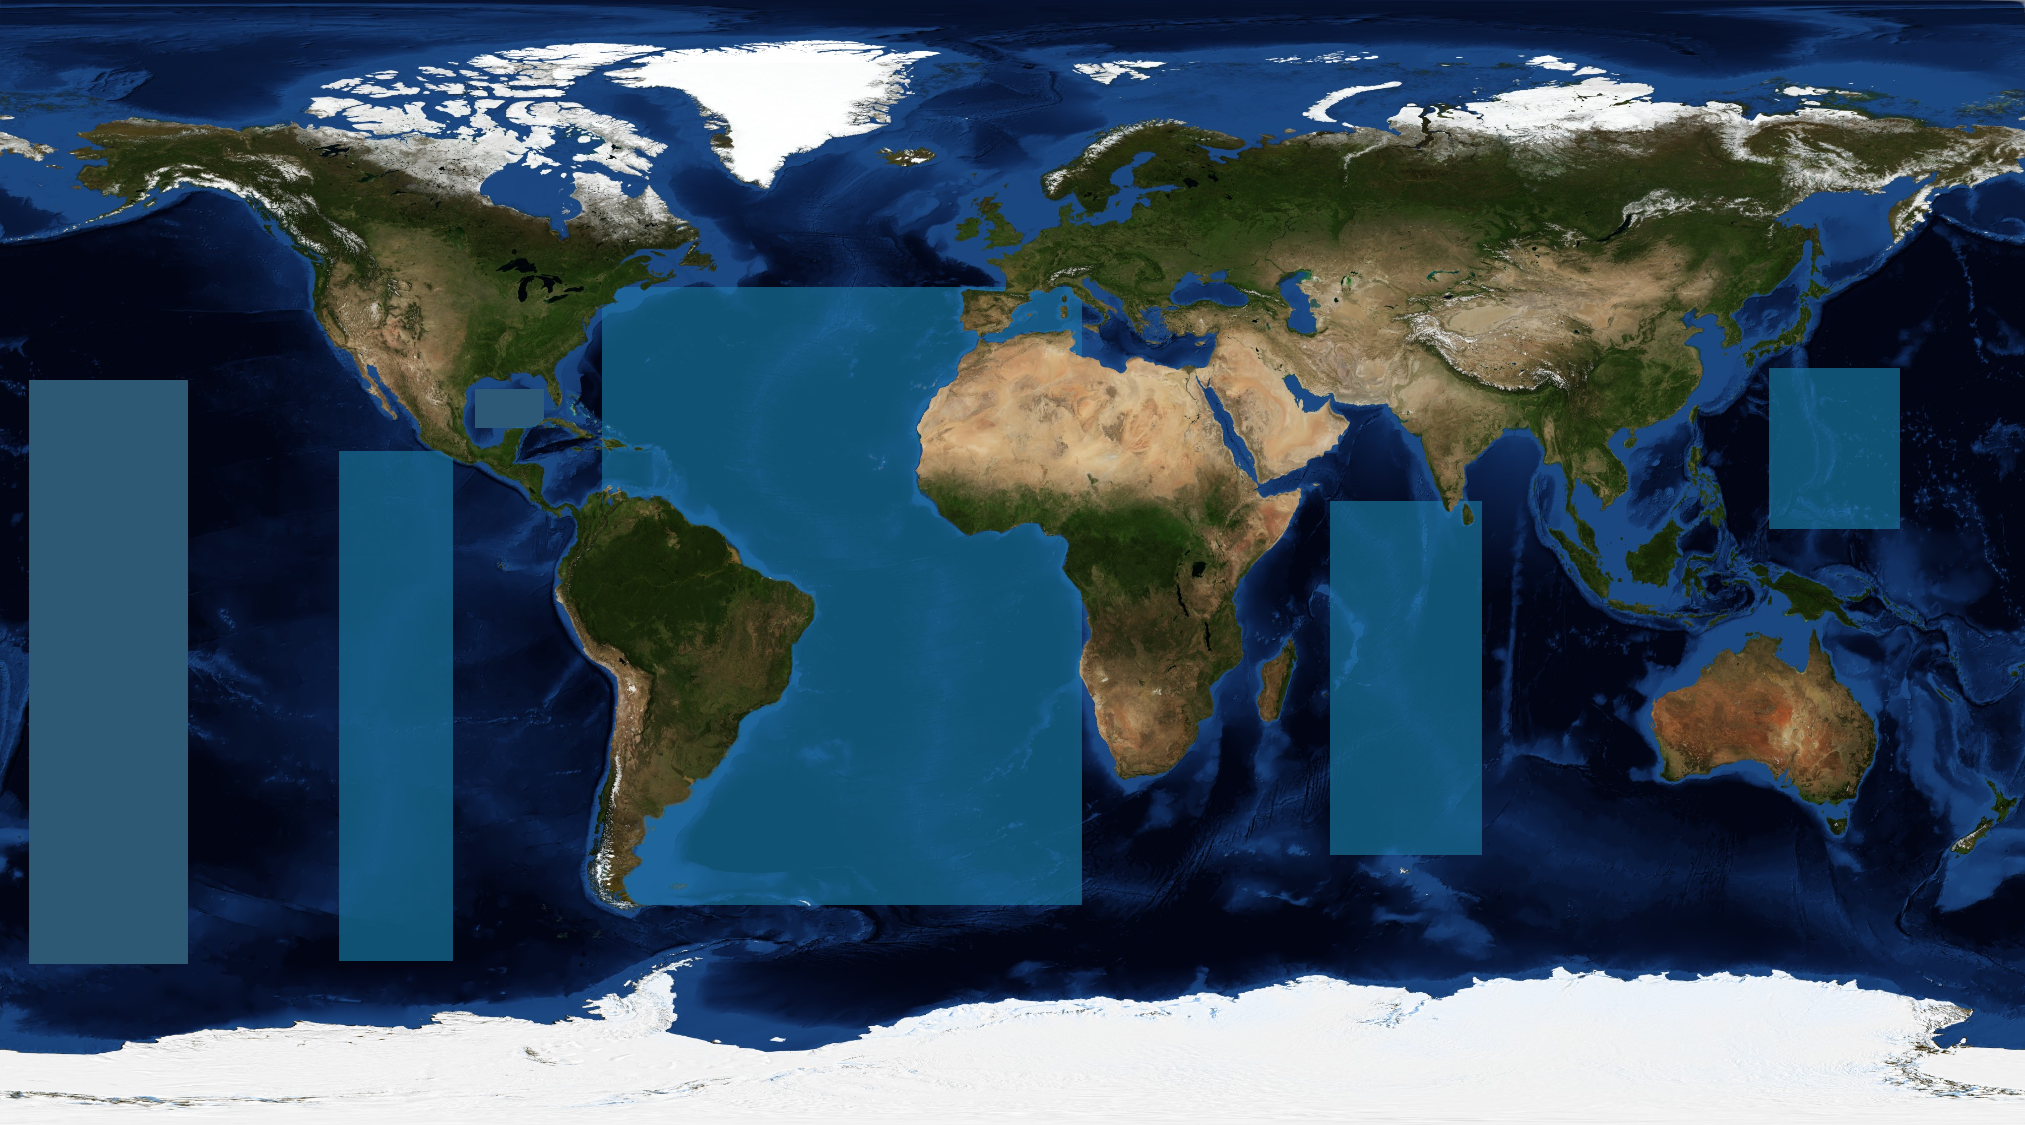
\includegraphics[width=\textwidth]{worldtraininglocal.png}
    \caption{Figure demonstrating initial training sets.}
    \label{fig:trainset}
\end{figure}

% \begin{table}[htb]
%     \centering
%     \begin{tabular}{|c c c|}
%         \hline
% 		\textbf{Model} & \textbf{\(R^2\)} & \textbf{RMSE} \\
% 		\hline
% 		SVM Regression & 0.841 & 365.23m \\
% 		Naive Bayes & 0.884 & 294.92m \\
%         Linear Regression & 0.885 & 265.43m \\
% 	    \hline
%     \end{tabular}
%     \label{table:REGRESSION_RESULTS}
%     \caption{Regression Results}
% \end{table}

\begin{figure}[]
    \centering
    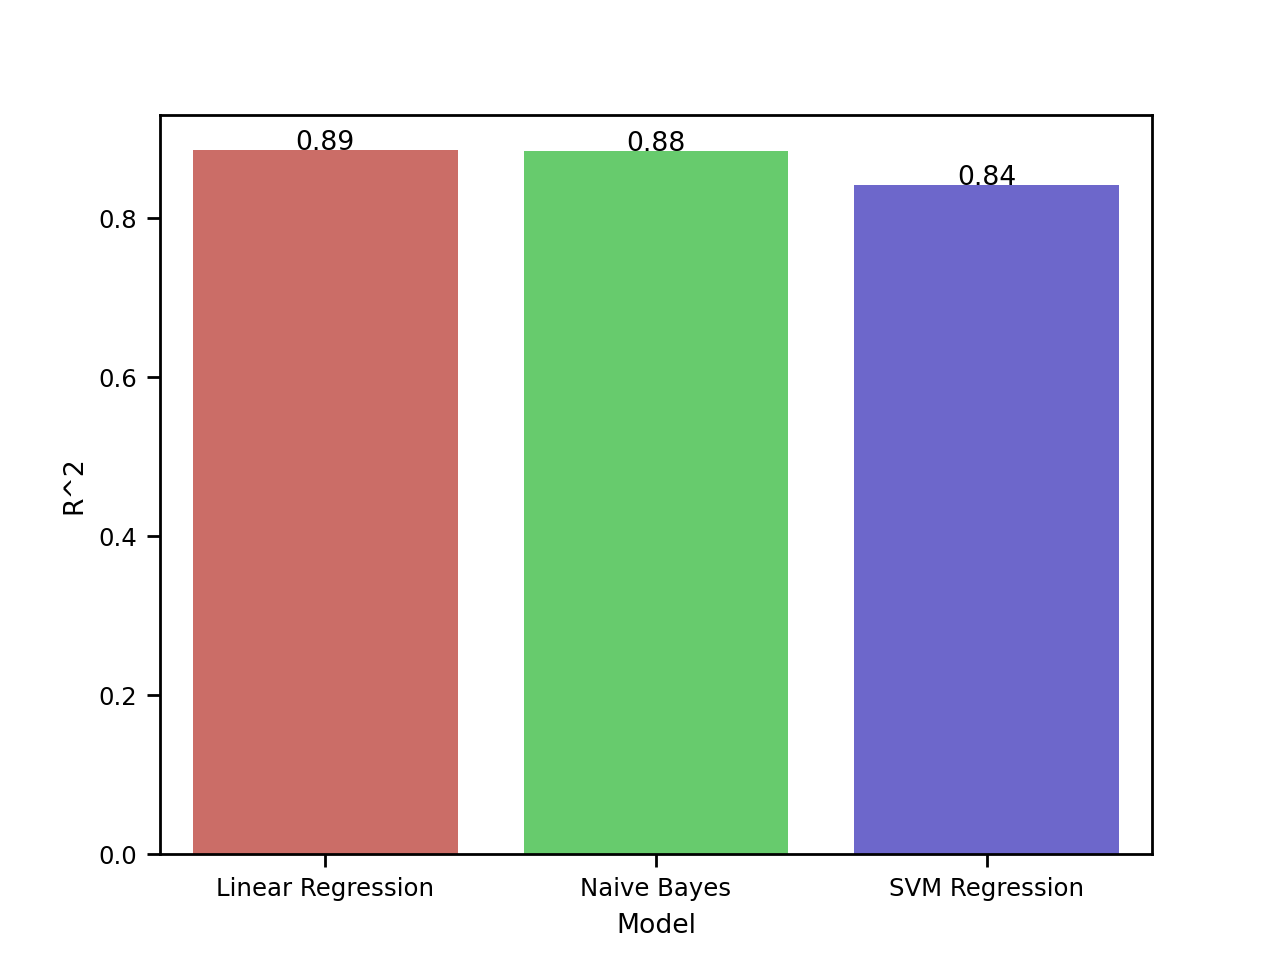
\includegraphics[scale=0.5]{rsquared_barplot_regression.png}
    \caption{Bar chart showing \(R^2\) score for each model}
    \label{fig:r2_barplot_regression}
\end{figure}

\begin{figure}[]
    \centering
    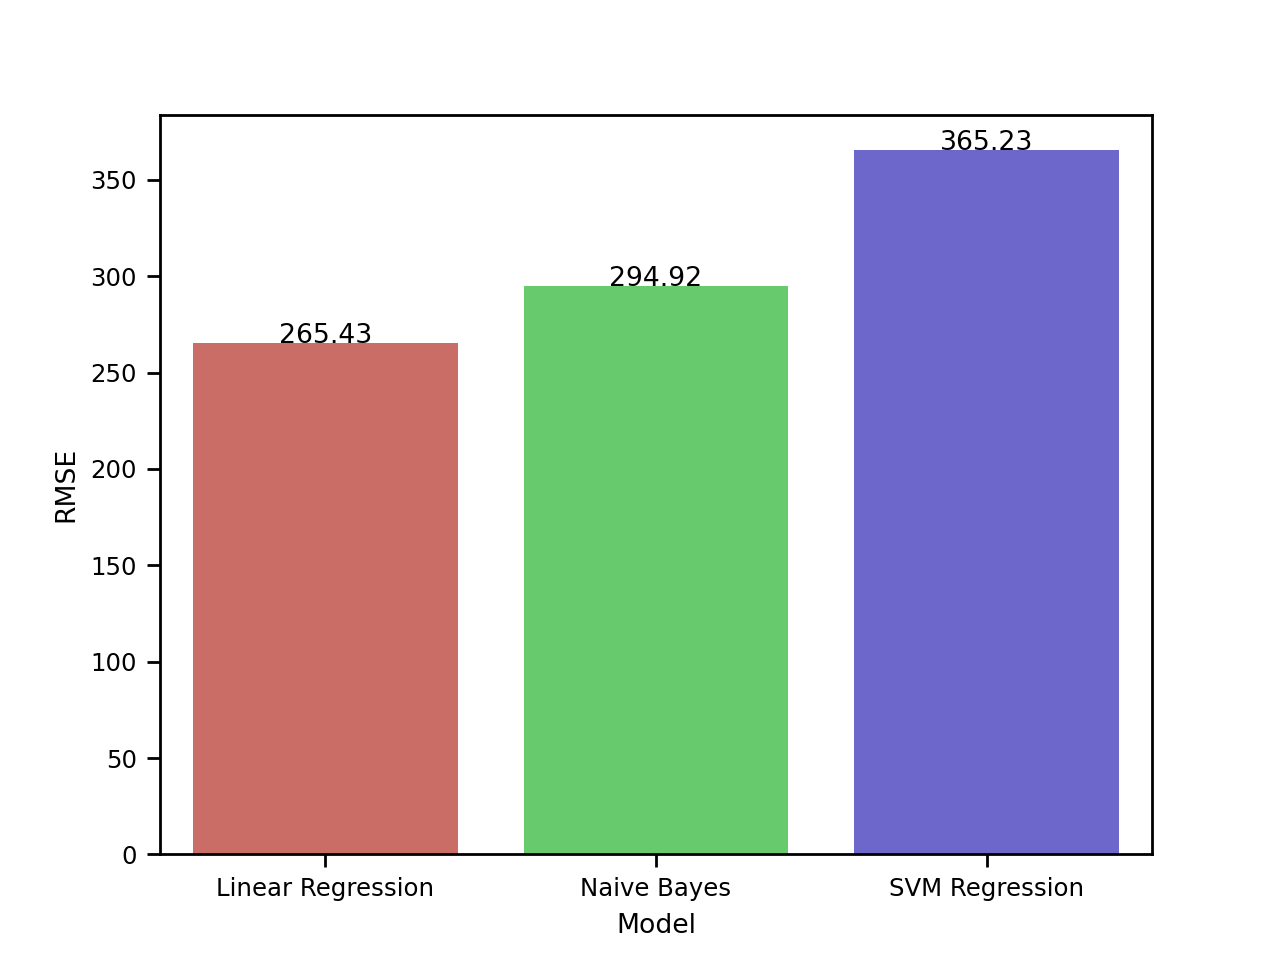
\includegraphics[scale=0.5]{rmse_bar_regression.png} 
    \caption{Bar chart showing RMSE for each model}
    \label{fig:rmse_barplot_regression}
\end{figure}

% \subsubsection{Regression Results Discussion}
% \cite{jena2012prediction} achieved a \ac{RMSE} of \~{}175m in their optimized model.
% The linear regression model I fit is 100 meters less accurate than the optimized model used in \cite{jena2012prediction}.
% However, the purpose of the test is not to achieve accurate predictions, but to identify if \ac{ML} models can be viable.
% Therefore, the accuracy of these models is less important than identifying the viability of the models.
% The training data used is essentially predicted bathymetry, but shows that fitting a model to true bathymetry will yield a similar result.
% Analyizing the \(R^2\) score gives evidence of the viability of the model.
% This score suggests that there are underlying relationships in the model that can be used to train a successful model.

\subsection{Classification Results}
\setlength{\parindent}{10ex}
%Maybe reword this opening chapter???
In order to iterate on the results displayed in the previous chapter this problem was converted from a continuous prediction to a classification problem.
Conversion was executed by mapping the bathymetry values into discrete classes.
This conversion proved to be trivial because of the ordered nature of bathymetry.
Classification models are simpler and easier to fit than regression models.
Idealy, the decision surfaces will benefit from the conversion and yield better results.
Classification models predict labels and not continuous values.
This makes it difficult to compare directly to the error reported in existing physics models.
A set of metrics including: precision, recall, f1 score, and balanced accuracy were used to analyize the viability of the models.

\par
The ordinal classes were binned on a interval of 150 meters.
This was done to easily compare accuracy to model in \cite{jena2012prediction}.
Validation was preformed using a 10 fold cross validation using balanced accuracy as the scoring function.

% \begin{table}[htb]
%     \centering
%     \begin{tabular}{|c c c|}
%         \hline
% 		\textbf{Model} & \textbf{Average F1 Score} & \textbf{Mean Balanced Accuracy} \\
% 		\hline
% 		Random Forest & 0.81 & 0.82 \\
%         Bagging & 0.80 & 0.79 \\
%         Decision Tree & 0.44 & 0.47 \\
%         \hline
%     \end{tabular}
%     \label{table:CLASSIFICATION_RESULTS}
%     \caption{Classification Results}
% \end{table}

\begin{figure}[]
    \centering
    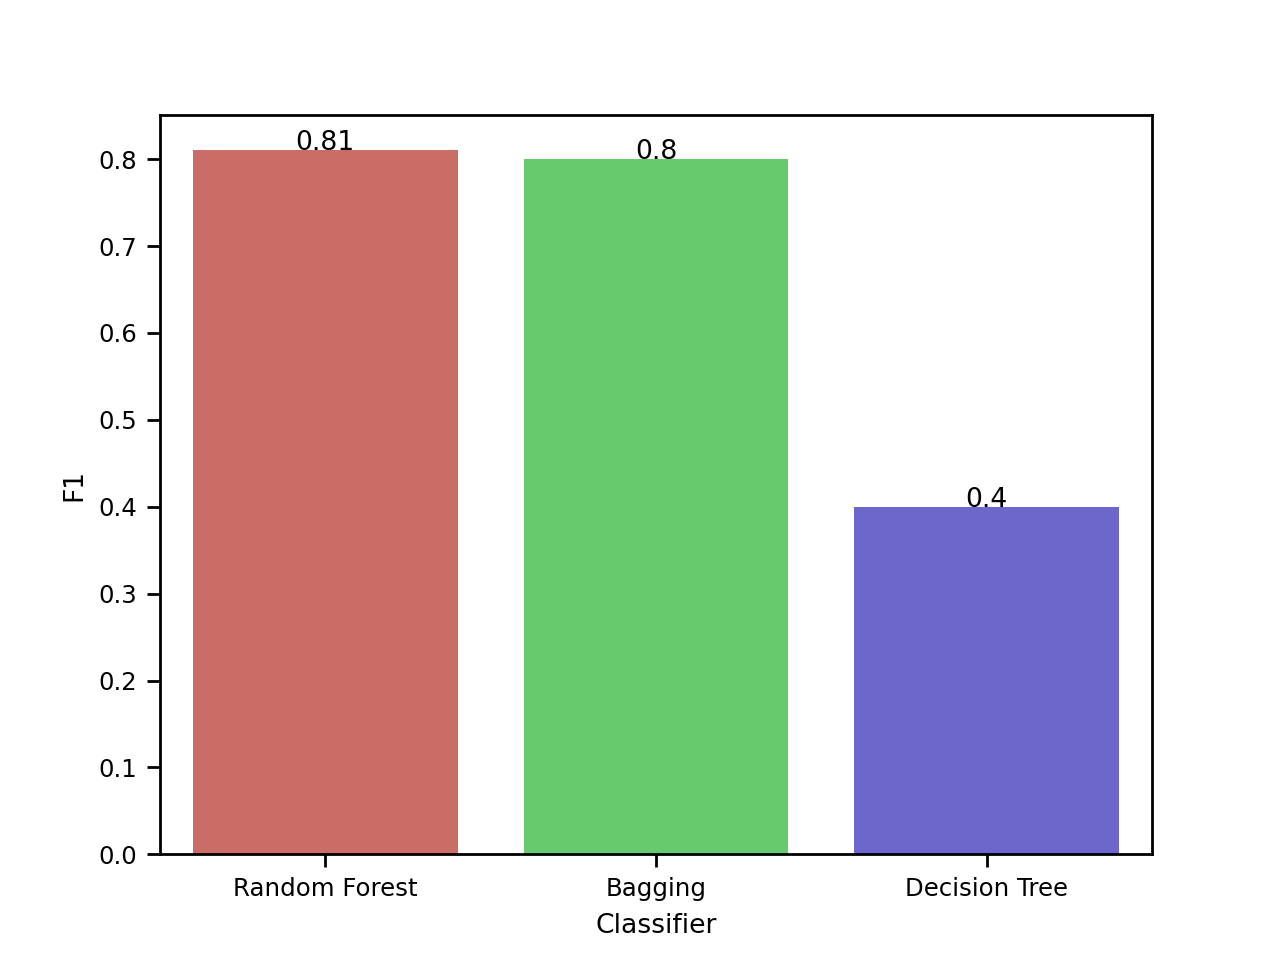
\includegraphics[scale=0.5]{f1_bar_classification.png}
    \caption{Bar chart showing F1 score for each classifier}
    \label{fig:f1_barplot_classification}
\end{figure}

\begin{figure}[]
    \centering
    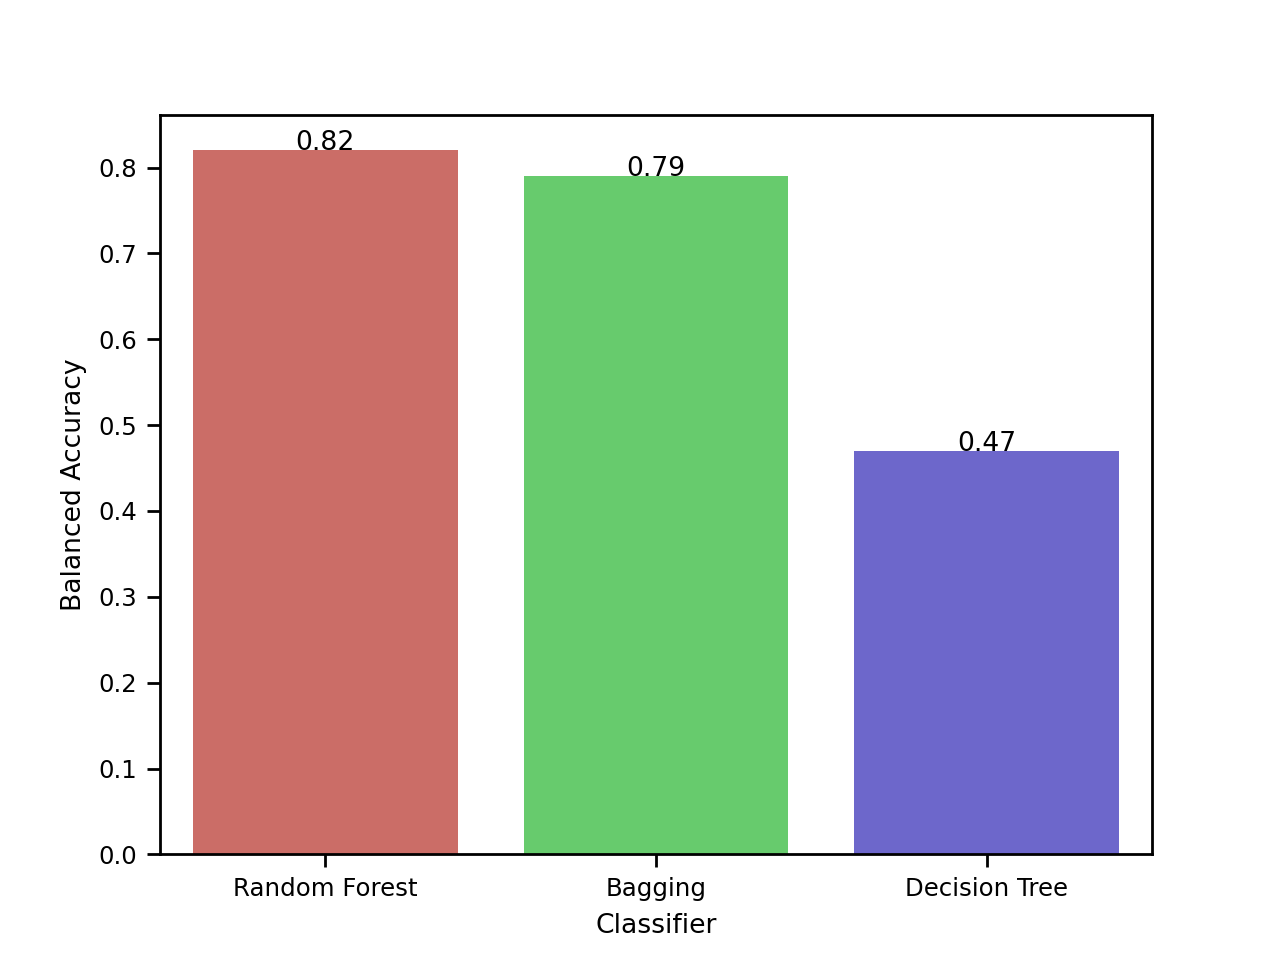
\includegraphics[scale=0.5]{balacc_bar_classification.png}
    \caption{Bar chart showing balanced accuracy for each classifier}
    \label{fig:balacc_barplot_classification}
\end{figure}

\subsection{Optimized Grid Model}
\setlength{\parindent}{10ex}
%Purpose of this section is to identify the optimized grid structure.
%I need to check with Hoque to identify what I should and shouldnt include
%I need to consider rewording this and restructuring to manage the correctness for example etc.
Further analysis of figure \ref{fig:rfc_report} shows that models are sensitive to potentially local characteristics.
In an attempt to test this notion and increase the accuracy of these models a novel model selection method was employed.
The objective being to identify if a model will predict more accuractly based on geospatial location.
The hypothysis being that decision boundaries across different models will respond to features based on location.

The Grid Optimized Model Injector Classifier was created to test this theory.
This model is built upon the idea that there is not a optimal single model for predicting all of the worlds bathymetry.
It leverages several different models to predict bathymetry in a area by recording the best preforming models across a grid of the world.
This allows the model to use the optimal model for predicting bathymetry.

\begin{figure}[]
    \centering
    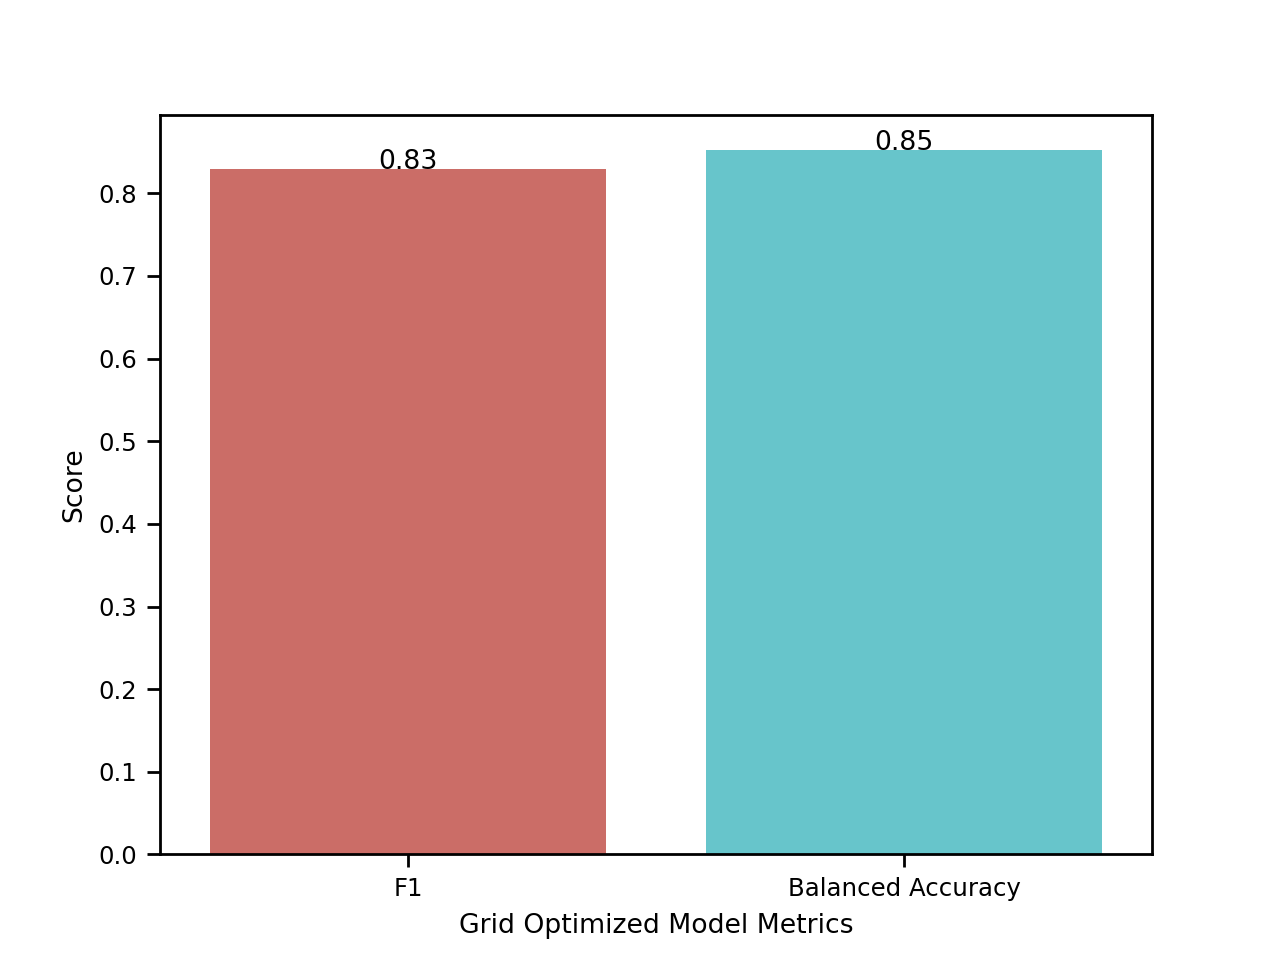
\includegraphics[scale=0.5]{grid_opt_results.png}
    \caption{Bar chart showing Grid Optimized Model results}
    \label{fig:grid_opt_barplot}
\end{figure}

%Give the background for the idea in this section!
\subsection{Analysis of Global Model Optimization}
Testing this hypothysis was performed by splitting the world into coverages.
Each coverage represented a exclusive area of the Earth's ocean.
A set of models were trained on each coverage and their prediction accuracies were compared.
The most accurate model was then saved for each coverage and stored in a map.
The results of this script are displayed in figure \ref{fig:coveragegrid}.

\begin{figure}[h]
    \centering
    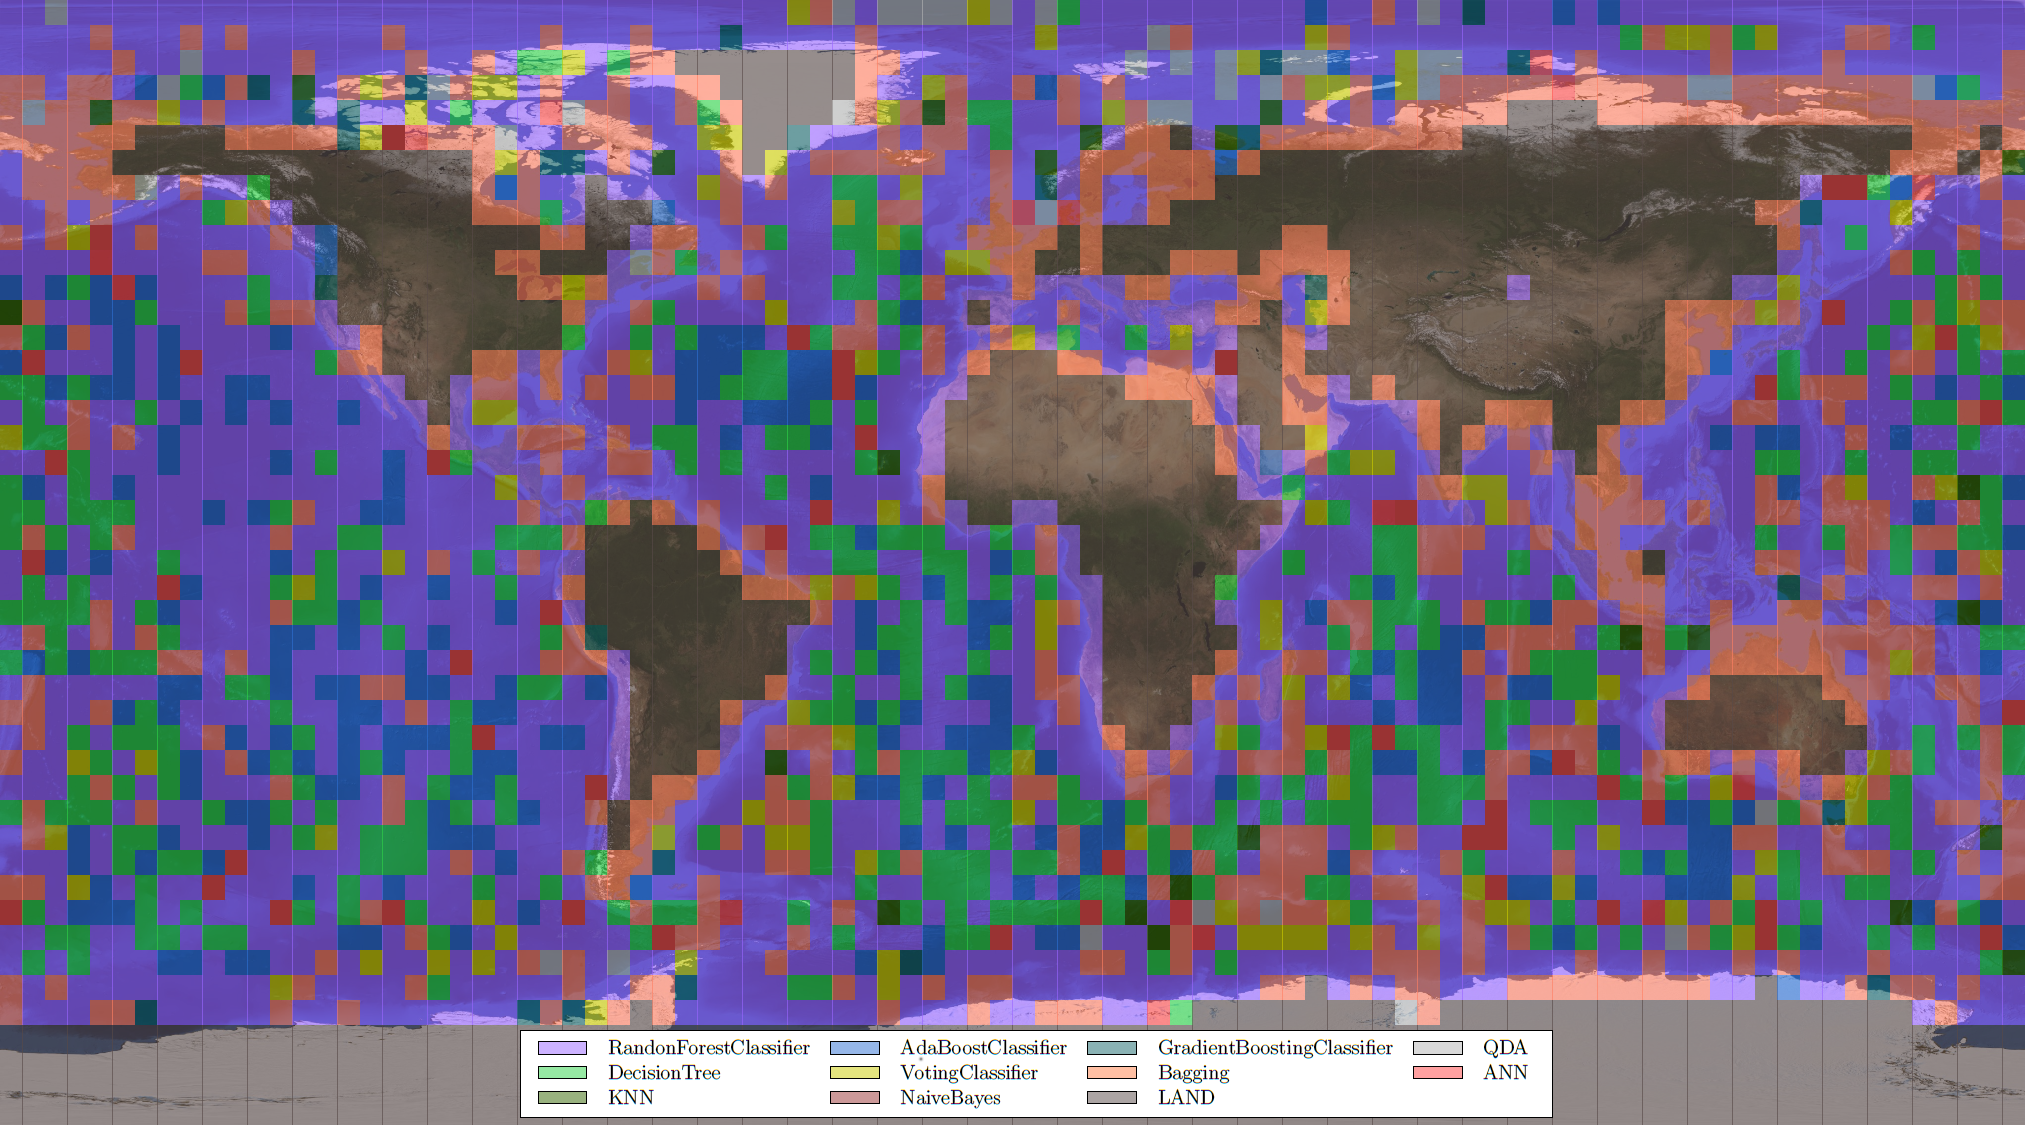
\includegraphics[width=\textwidth]{optgriddraft.png}
    \caption{Graphic Showing the World Coverages and Successful Models}
    \label{fig:coveragegrid}
\end{figure}

\par
Clearly, figure \ref{fig:coveragegrid} provides evidence that model decision boundaries are sensitive to the features based on location.
Leading to the conclusion that there is not a single best fit model for predicting global bathymetry.
Analysis of figure \ref{fig:coveragegrid} shows interesting consistencies that raise questions about the underlying features.
For example, the decision tree classifier preformed poorly as configured in the classification section when used for global predictions.
When predicting near fault lines it preformed the best out of other models.
Bagging seemed to dominate on coast lines while \ac{RFC} performed best in open waters.

%In this section I am defining what the Grid optimization is and why it matters.
%There may be a better name for this?? Who knows really...
\subsubsection{Grid Optimizing}
The results of the experiment were then used for model selection.
Using the successful model for each coverage as a \textit{optimum} selection.
A trivial geospatial query is used to query the best model by location.
This selection is implemented in a novel model I call the \textit{Grid Optimized Model Injector Classifier}.
This name is chosen because the result model acquired from the spatial query is injected for classification.

%This is where I define what happens after the appropriate coverages have been found.
\par
In theory, this injection will allow each model to perform to its optimum.
Each coverage highlights distinct characteristics that will produce a better decision boundary.
These coverages are simple partitions of the world, but could be extended in future work to optimize the selection.
% Reconsider this sentence....

